\documentclass[parskip=full, 12pt, oneside]{scrbook}

\usepackage[utf8]{inputenc} % use utf8 file encoding for TeX sources
\usepackage[T1]{fontenc} % avoid garbled Unicode text in pdf
\usepackage[english]{babel} % english hyphenation, quotes, etc
\usepackage[hidelinks]{hyperref} % detailed hyperlink/pdf configuration
\usepackage{csquotes}
\usepackage{authblk}
\usepackage{enumitem}
\usepackage{graphicx} %%provides the  \includegraphics macro
\usepackage{float} %%provides the H directive to force position of figures (\begin{figure}[H])
\usepackage[numberedsection,nonumberlist,toc,section=chapter]{glossaries}     % provides glossary commands
\usepackage{scrhack} %%make above float package compatible with komascript
\usepackage{ifthenx}
\usepackage{intcalc}
\hypersetup{ % `texdoc hyperref` for options
	pdftitle={Software Design},
	bookmarks=true,
}

\makenoidxglossaries

% Configure Title Page Layout
\subject{Karlsruhe Institute of Technology}
\author{
	\textit{Irma Suppes, Karl Rubel, } \\ 
	\textit{Mingyi Li, Niklas Bülow, Sönke Jendral }
}
\title{MORR \\ (Medical Online Research Recorder)}
\subtitle{PSE-Project \\ Software design}
\publishers{Supervisors: \\ \textit{Paula Breitling, Dr. Till Riedel, Tobias Röddiger}}

\chapter{Glossary}
\label{ch:glossary}

\begin{document}


\maketitle

\chapter*{Document Version History}
\label{ch:versionhistory}
\begin{table}[h]
\begin{tabular}{lll}
\textbf{Revision} & \textbf{Date} & \textbf{Description}              \\
\hline
1.0.0             & 13.12.2019    & Creation and release of document. \\
\hline
1.1.0			  & 14.02.2020	  & Update software-design: \\
&& Update BrowserExtension Shared section\\
&& (Update EventType enum and serialize method)\\
&& Update BrowserExtension Background section\\
&& (Update methods of BackgroundScript and ICommunicationInterface)\\
&& Update BrowserExtension Listeners section\\
&& (Update factory methods)\\
&& Update BrowserExtension Content section\\
&& (Update method signature in DOMEventFactory)\\
&& Update ClipboardModule section\\
&& (Update producers methods, add new ClipboardEvents)\\
&& Update KeyboardModule section\\
&& (Update producers methods, update attributes in KeyboardInteractEvent)\\
&& Update MouseModule section\\
&& (Update producers methods, add MouseModuleConfiguration,\\
&& update attributes in mouse events)\\
&& Update WebBrowserModule section\\
&& (Update producers methods, add WebBrowserModuleConfiguration,\\
&& add classes for communication with WebExtension,\\
&& add WebBrowserProducer abstract class)\\
&& Update WindowManagementModule section\\
&& (Update producers methods)\\

\end{tabular}
\end{table}% History of document versions
\tableofcontents
\chapter{Introduction}
\label{ch:introduction}    % Introduction
\chapter{Application Data}
\label{ch:data}
    % Architecture
\chapter{Directory structure}
\label{ch:dirstructure}

\dirtree{%
.1 application.
	.2 BrowserExtension.
		.3 materials.
			.4 logos.
		.3 src.
			.4 ApplicationInterface.
			.4 Listeners.
				.5 DOM.
					.6 ContentScript.
				.5 Download.
				.5 Tab.
			.4 Shared.
	.2 Common.
		.3 Shared.
			.4 Configuration.
			.4 Events.
				.5 Queue.
					.6 Strategy.
						.7 MultiConsumer.
						.8 SingleConsumer.
			.4 Hook.
				.5 Exceptions.
			.4 Modules.
			.4 Utility.
		.3 HookLibrary.
		.3 Win32HookHelper.
	.2 Core.
		.3 CLI.
			.4 Commands.
				.5 Processing.
				.5 Recording.
				.5 Validate.
			.4 Interactive.
			.4 Output.
			.4 Utility.
		.3 MORR.
			.4 Configuration.
			.4 Data.
				.5 Capture.
					.6 Video.
						.7 Desktop.
							.8 Utility.
						.7 Exceptions.
				.5 IntermediateFormat.
					.6 Json.
				.5 Transcoding.
					.6 Exceptions.
					.6 Json.
					.6 MPEG.
					.6 Video.
						.7 Exceptions.
			.4 Modules.
			.4 Session.
				.5 Crypto.
				.5 Exceptions.
		.3 UI.
			.4 Assets.
				.5 Icon.
			.4 Controls.
				.5 NotifyIcon.
			.4 Dialogs.
			.4 Styles.
			.4 Utility.
			.4 ViewModels.
	.2 Modules.
		.3 Clipboard.
			.4 Events.
			.4 Native.
			.4 Producers.
		.3 Keyboard.
			.4 Events.
			.4 Native.
			.4 Producers.
		.3 Mouse.
			.4 Events.
			.4 Native.
			.4 Producers.
		.3 WebBrowser.
			.4 Events.
			.4 Producers.
		.3 WindowManagement.
			.4 Events.
			.4 Native.
			.4 Producers.
}    % Directory structure
\chapter{Packages}
\label{ch:package}
\newenvironment{packclass}[0]{\textbf{Contained classes:} \begin{itemize}
}{\end{itemize}}
\newenvironment{packenum}[0]{\textbf{Contained enums:} \begin{itemize}
}{\end{itemize}}
\newenvironment{packif}[0]{\textbf{Contained interfaces:} \begin{itemize}
}{\end{itemize}}
\newenvironment{packpack}[0]{\textbf{Contained packages:} \begin{itemize}
}{\end{itemize}}
\newcommand{\packobj}[1]{\item #1}
\newcommand{\abstract}[1]{\textit{abstract} #1}

In this chapter, all packages and their purpose are introduced.

\section{MORR}

\begin{center}
    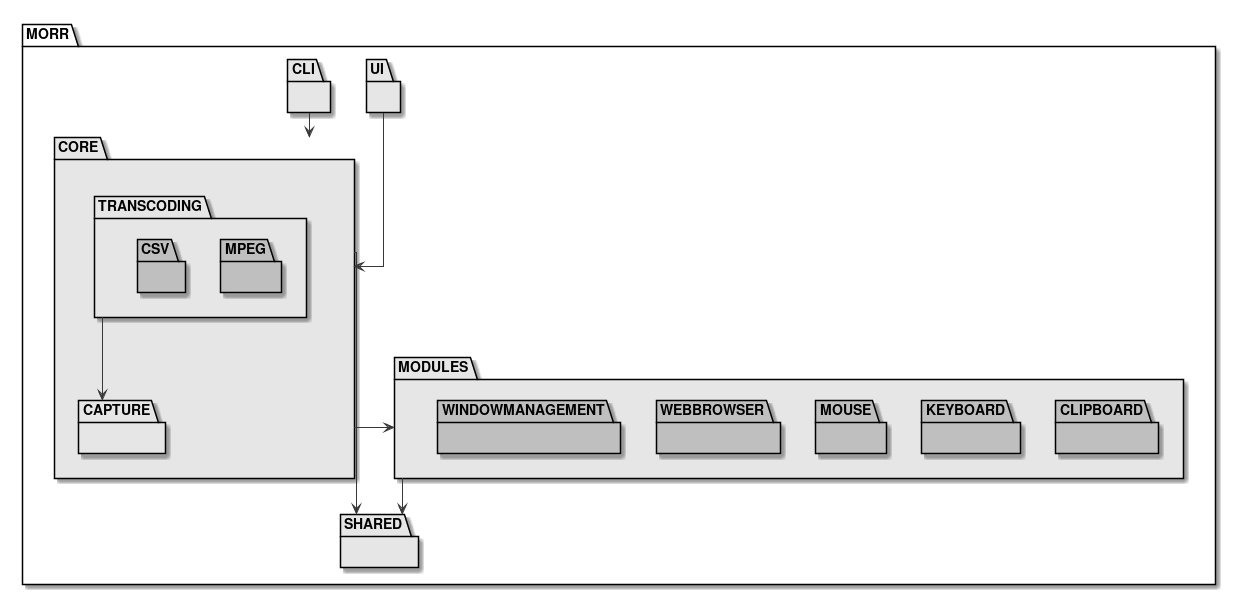
\includegraphics[width=0.80\textwidth]{resources/Packages/AllPackages.png}
\end{center}

The \textbf{MORR} package is the master package containing the whole application. It does not contain any classes directly as it only serves as a container for all packages required in the design.

\begin{packpack}
\packobj{CORE}
\packobj{CLI}
\packobj{SHARED}
\packobj{MODULES}
\packobj{UI}
\end{packpack}

\newpage
\section{MORR.CORE}

\begin{center}
    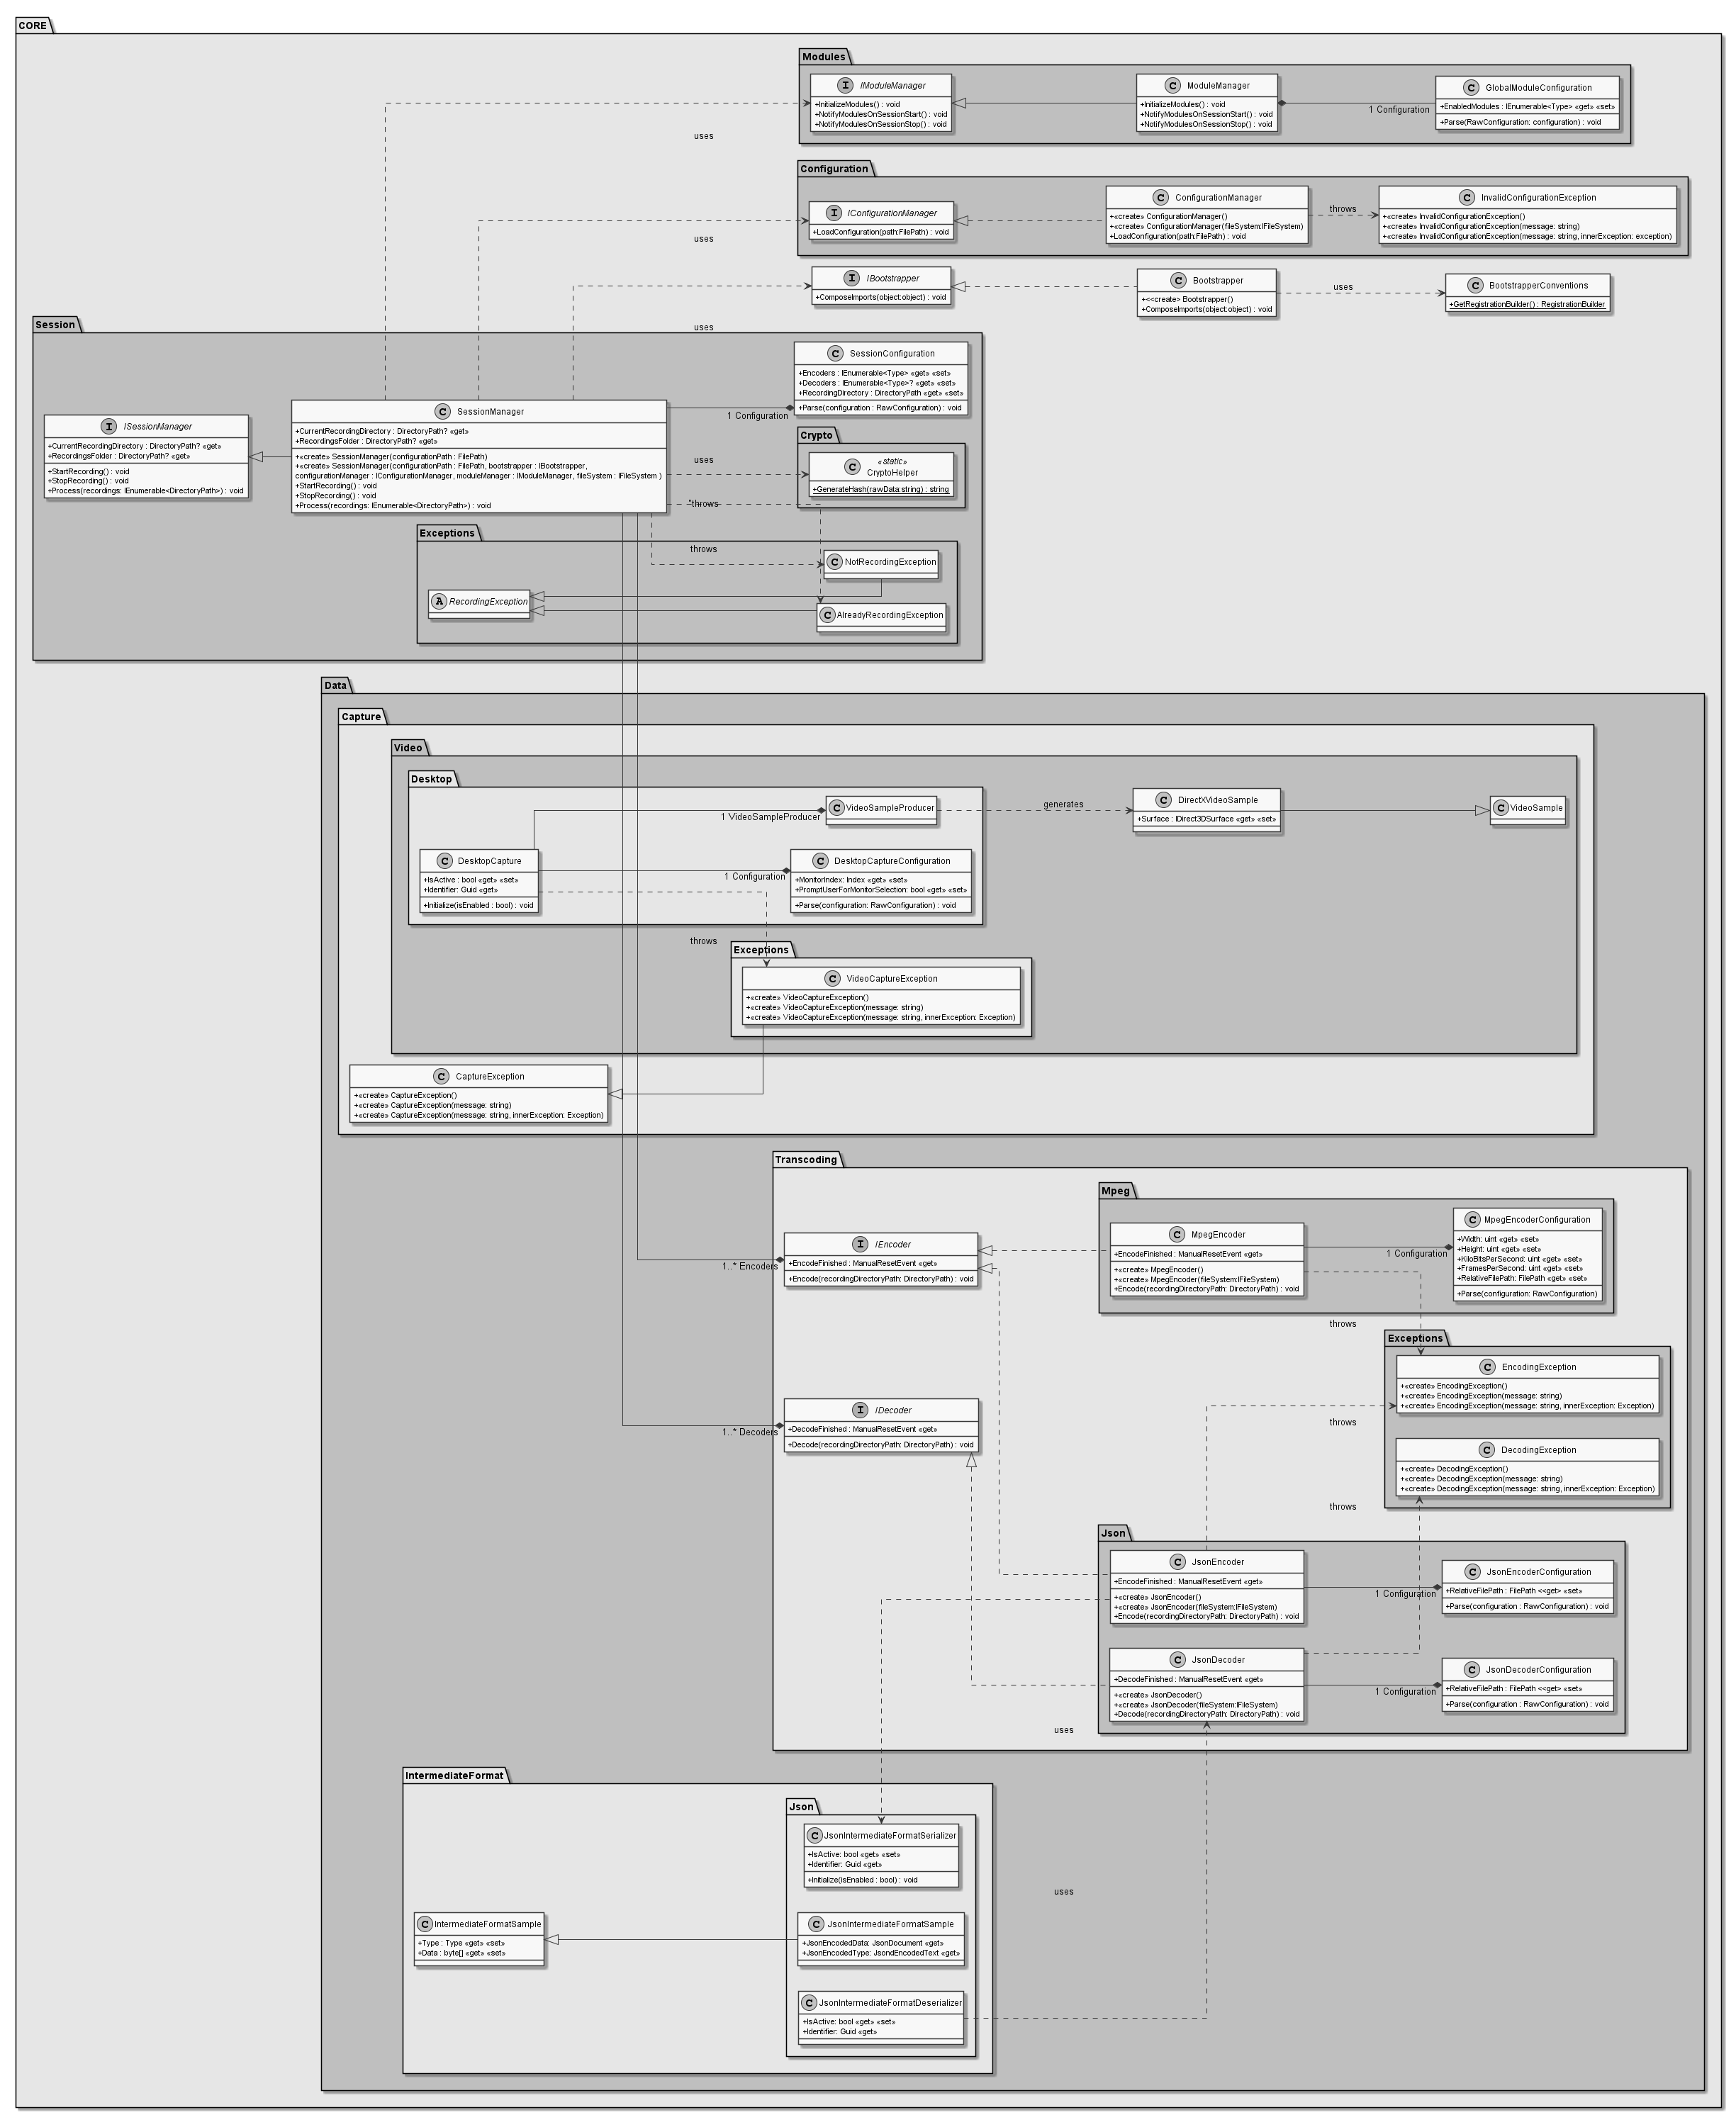
\includegraphics[width=1.0\textwidth]{resources/Packages/CORE.png}
\end{center}

The \textbf{CORE} package contains the central initializing logic to be called when the program is started and coordinates state-changes while the application is running.

\begin{packif}
\packobj{IModuleManager}
\packobj{IBootstrapper}
\packobj{IConfigurationManager}
\packobj{ISessionManager}
\end{packif}

\begin{packclass}
\packobj{SessionManager}
\packobj{Bootstrapper}
\packobj{ModuleManager}
\packobj{ConfigurationManager}
\packobj{RecordingException}
\packobj{InvalidConfigurationException}
\packobj{AlreadyRecordingException}
\packobj{NotRecordingException}
\packobj{GlobalModuleConfiguration}
\end{packclass}

\begin{packpack}
\packobj{TRANSCODING}
\packobj{CAPTURE}
\end{packpack}

\section*{MORR.CORE.TRANSCODING}

The \textbf{CORE.TRANSCODING} package is responsible for serialization and deserialization of recorded video-, audio- and event-data.

\begin{packif}
\packobj{IDecoder}
\packobj{IEncoder}
\packobj{IMetadataDeserializer}
\end{packif}

\begin{packclass}
\packobj{\abstract{VideoSample}}
\packobj{\abstract{MetadataSample}}
\packobj{DecodingException}
\packobj{EncodingException}
\packobj{CaptureException}
\packobj{IntermediateFormatSample}
\packobj{IntermediateFormatSerializer}
\packobj{IntermediateFormatDeserializer}
\packobj{JsonIntermediateFormatSample}
\packobj{VideoCaptureException}
\packobj{VideoSample}
\packobj{MonitorEnumerationHelper}
\end{packclass}

\begin{packpack}
\packobj{CSV}
\packobj{MPEG}
\end{packpack}

\section*{MORR.CORE.TRANSCODING.Json}
The \textbf{CORE.TRANSCODING.Json} package is responsible for providing functionality which allows for encoding of event data to Json format.

\begin{packclass}
\packobj{JsonEncoder}
\packobj{JsonDecoder}
\end{packclass}

\section*{MORR.CORE.TRANSCODING.MPEG}
The \textbf{CORE.TRANSCODING.MPEG} package allows for storing video-, audio- and event-data in a MPEG container and also retrieving this data again from such a container.

\begin{packclass}
\packobj{MPEGDecoder}
\packobj{MPEGDecoderConfiguration}
\end{packclass}

\section*{MORR.CORE.CAPTURE}

The \textbf{CORE.CAPTURE} package is responsible for capturing and supplying samples to the encoders.

\begin{packif}
\packobj{IVideoCapture}
\packobj{IMetadataCapture}
\end{packif}

\begin{packclass}
\packobj{DesktopCapture}
\packobj{DesktopCaptureConfiguration}
\packobj{CaptureHelper}
\packobj{Direct3D11Helper}
\packobj{DirectXVideoSample}
\packobj{CaptureException}
\packobj{VideoCaptureException}
\end{packclass}

\newpage
\section{MORR.CLI}

\begin{center}
    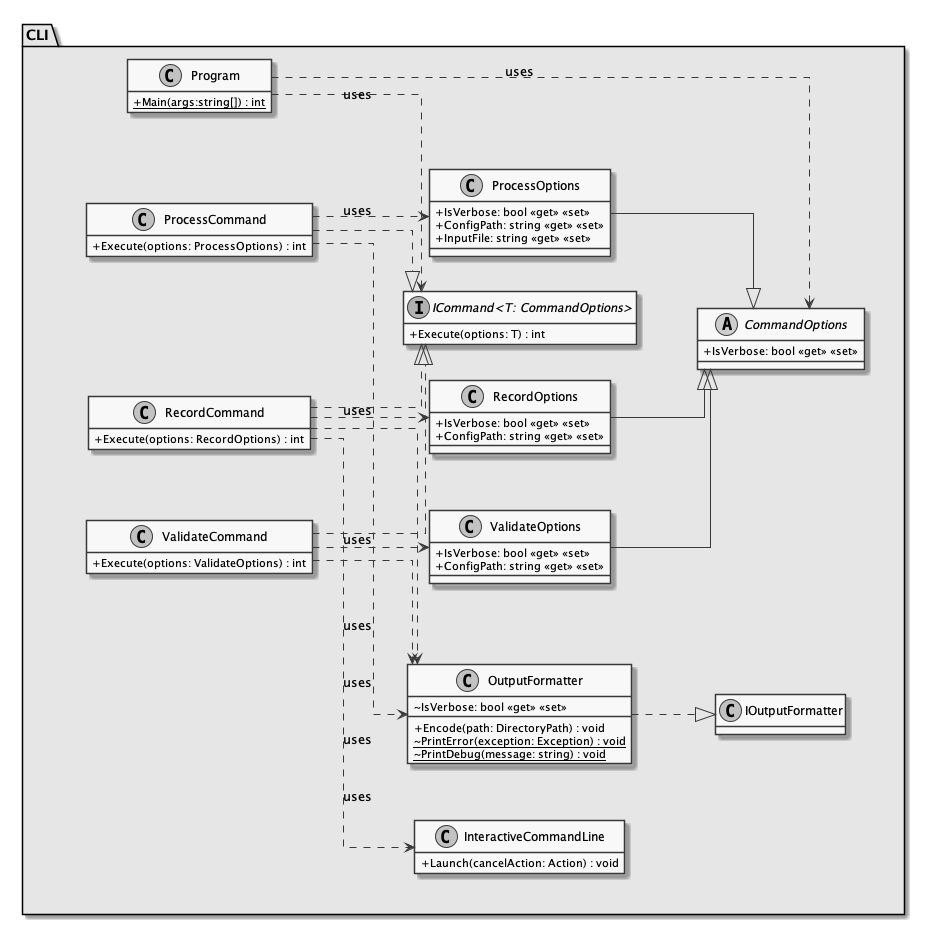
\includegraphics[width=1.0\textwidth]{resources/Packages/CLI.png}
\end{center}

The \textbf{CLI} package contains all logic exclusively needed for the command line interface which allows for the extraction of event data from saved recordings.

\begin{packif}
\packobj{ICommand<T: CommandOptions>}
\packobj{IOutputFormatter}
\end{packif}

\begin{packclass}
\packobj{OutputFormatter}
\packobj{CommandOptions}
\packobj{RecordCommand}
\packobj{RecordOptions}
\packobj{ValidateCommand}
\packobj{ValidateOptions}
\packobj{ProcessCommand}
\packobj{ProcessOptions}
\packobj{InteractiveCommandLine}
\packobj{ProcessOptions}
\packobj{Program}
\end{packclass}

\newpage
\section{MORR.SHARED}

\begin{center}
    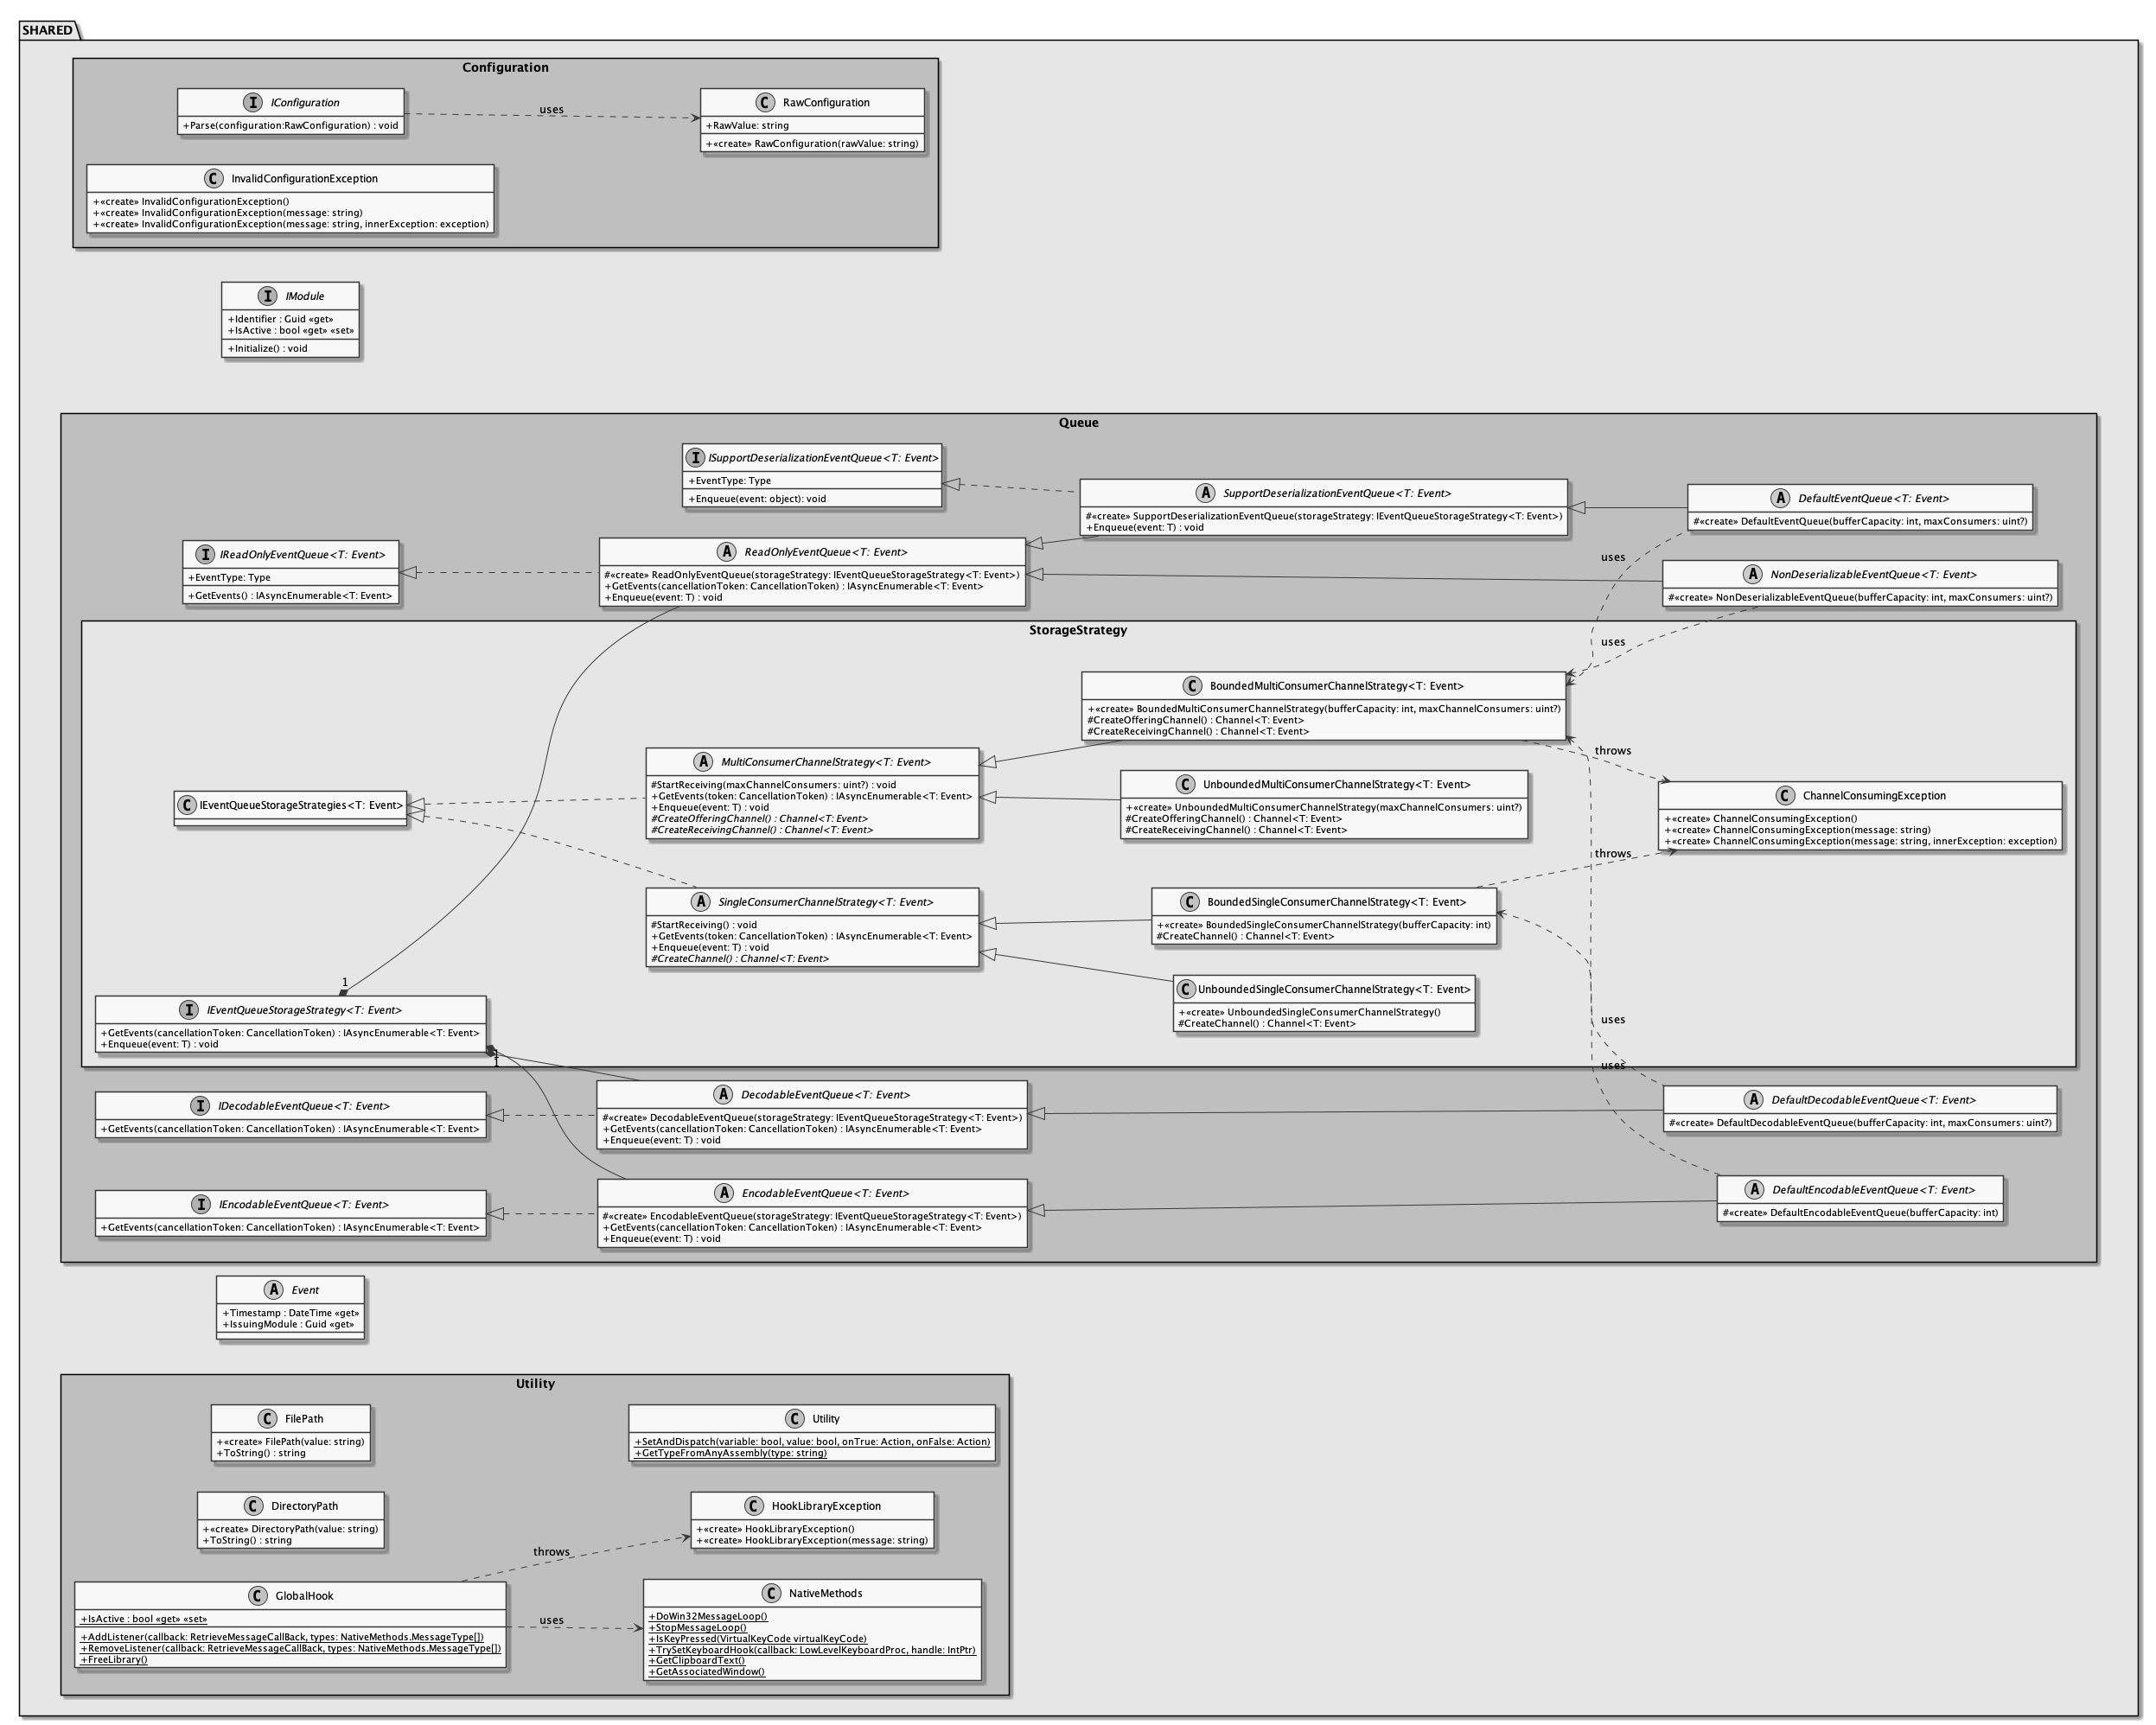
\includegraphics[width=1.0\textwidth]{resources/Packages/SHARED.png}
\end{center}

The \textbf{SHARED} package provides interfaces and classes which have to be known and shared across multiple packages, such as the concept of an event or a module.

\begin{packif}
\packobj{IConfiguration}
\packobj{IModule}
\packobj{IReadOnlyEventQueue<T: Event>}
\packobj{ISupportDeserializationEventQueue<T: Event>}
\packobj{IEventQueueStorageStrategy<T: Event>}
\packobj{IDecodableEventQueue<T: Event>}
\packobj{IEncodableEventQueue<T: Event>}
\end{packif}

\begin{packclass}
\packobj{RawConfiguration}
\packobj{\abstract{Event}}
\packobj{InvalidConfigurationException}
\packobj{\abstract{ReadOnlyEventQueue<T: Event>}}
\packobj{\abstract{SupportDeserializationEventQueue<T: Event>}}
\packobj{DefaultEventQueue<T: Event>}
\packobj{NonDeserializableEventQueue<T: Event>}
\packobj{\abstract{MultiConsumerChannelStrategy<T: Event>}}
\packobj{\abstract{SingleConsumerChannelStrategy<T: Event>}}
\packobj{BoundedMultiConsumerChannelStrategy<T: Event>}
\packobj{UnboundedMultiConsumerChannelStrategy<T: Event>}
\packobj{BoundedSingleConsumerChannelStrategy<T: Event>}
\packobj{UnboundedSingleConsumerChannelStrategy<T: Event>}
\packobj{ChannelConsumingException}
\packobj{\abstract{DecodableEventQueue<T: Event>}}
\packobj{\abstract{EncodableEventQueue<T: Event>}}
\packobj{DefaultEncodableEventQueue<T: Event>}
\packobj{DefaultDecodableEventQueue<T: Event>}
\packobj{FilePath}
\packobj{DirectoryPath}
\packobj{GlobalHook}
\packobj{Utility}
\packobj{HookLibraryException}
\packobj{NativeMethods}
\end{packclass}

\newpage
\section{MORR.MODULES}

The \textbf{MODULES} package serves as a container for all module-subpackages.

\begin{packpack}
\packobj{WINDOWMANAGEMENT}
\packobj{KEYBOARD}
\packobj{CLIPBOARD}
\packobj{WEBBROWSER}
\packobj{MOUSE}
\end{packpack}

\subsection*{MORR.MODULES.WINDOWMANAGEMENT}

\begin{center}
    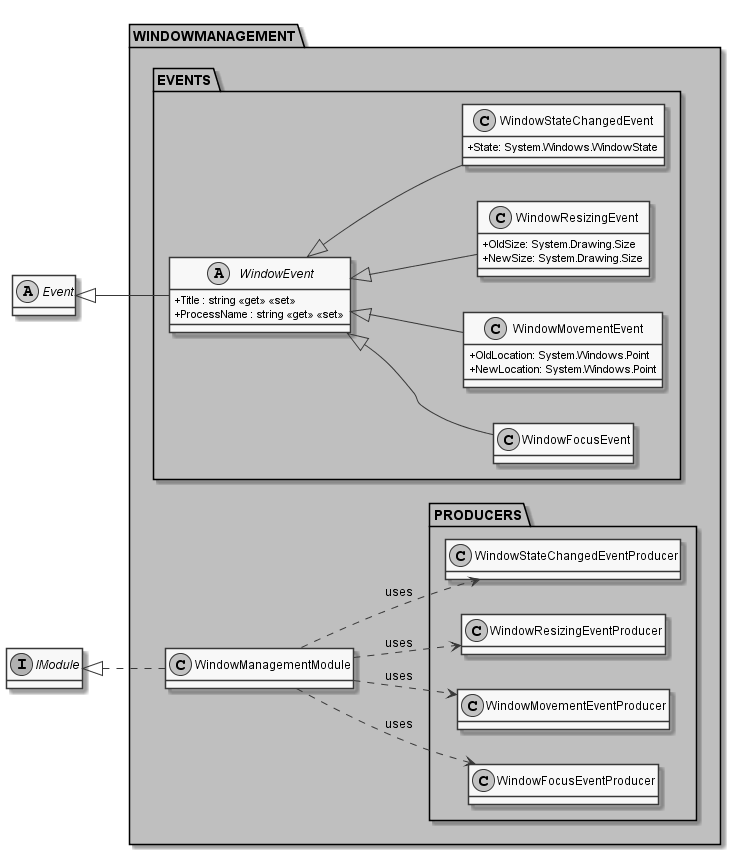
\includegraphics[width=1.0\textwidth]{resources/Packages/MODULES_WINDOWMANAGEMENT.png}
\end{center}

The \textbf{MODULES.WINDOWMANAGEMENT} package is responsible for providing the classes and concepts necessary for recording the window related user-interactions.

\begin{packclass}
\packobj{WindowManagementModule}
\packobj{\abstract{WindowEvent}}
\packobj{WindowMovementEvent}
\packobj{WindowFocusEvent}
\packobj{WindowSateChangedEvent}
\packobj{WindowResizingEvent}
\end{packclass}
\newpage
\subsection*{MORR.MODULES.KEYBOARD}

\begin{center}
    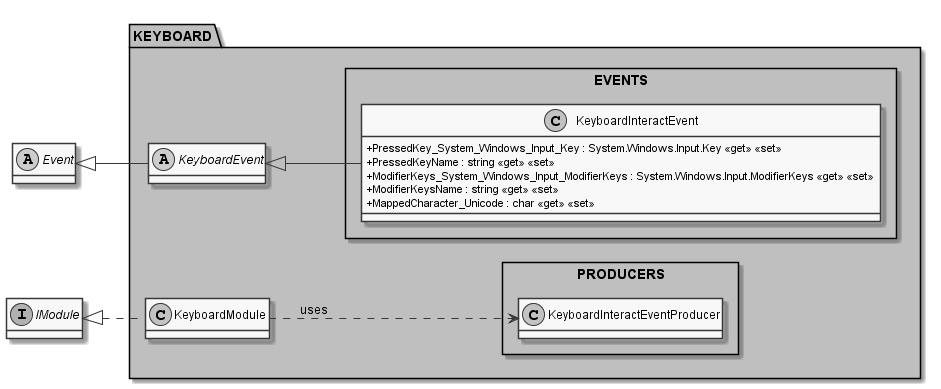
\includegraphics[width=1.0\textwidth]{resources/Packages/MODULES_KEYBOARD.png}
\end{center}

The \textbf{MODULES.KEYBOARD} package is responsible for providing the classes and concepts necessary for recording the keyboard related user-inputs.

\begin{packclass}
\packobj{\abstract{KeyboardEvent}}
\packobj{KeyboardModule}
\packobj{KeyboardInteractEvent}
\end{packclass}

\newpage
\subsection*{MORR.MODULES.WEBBROWSER}

\begin{center}
    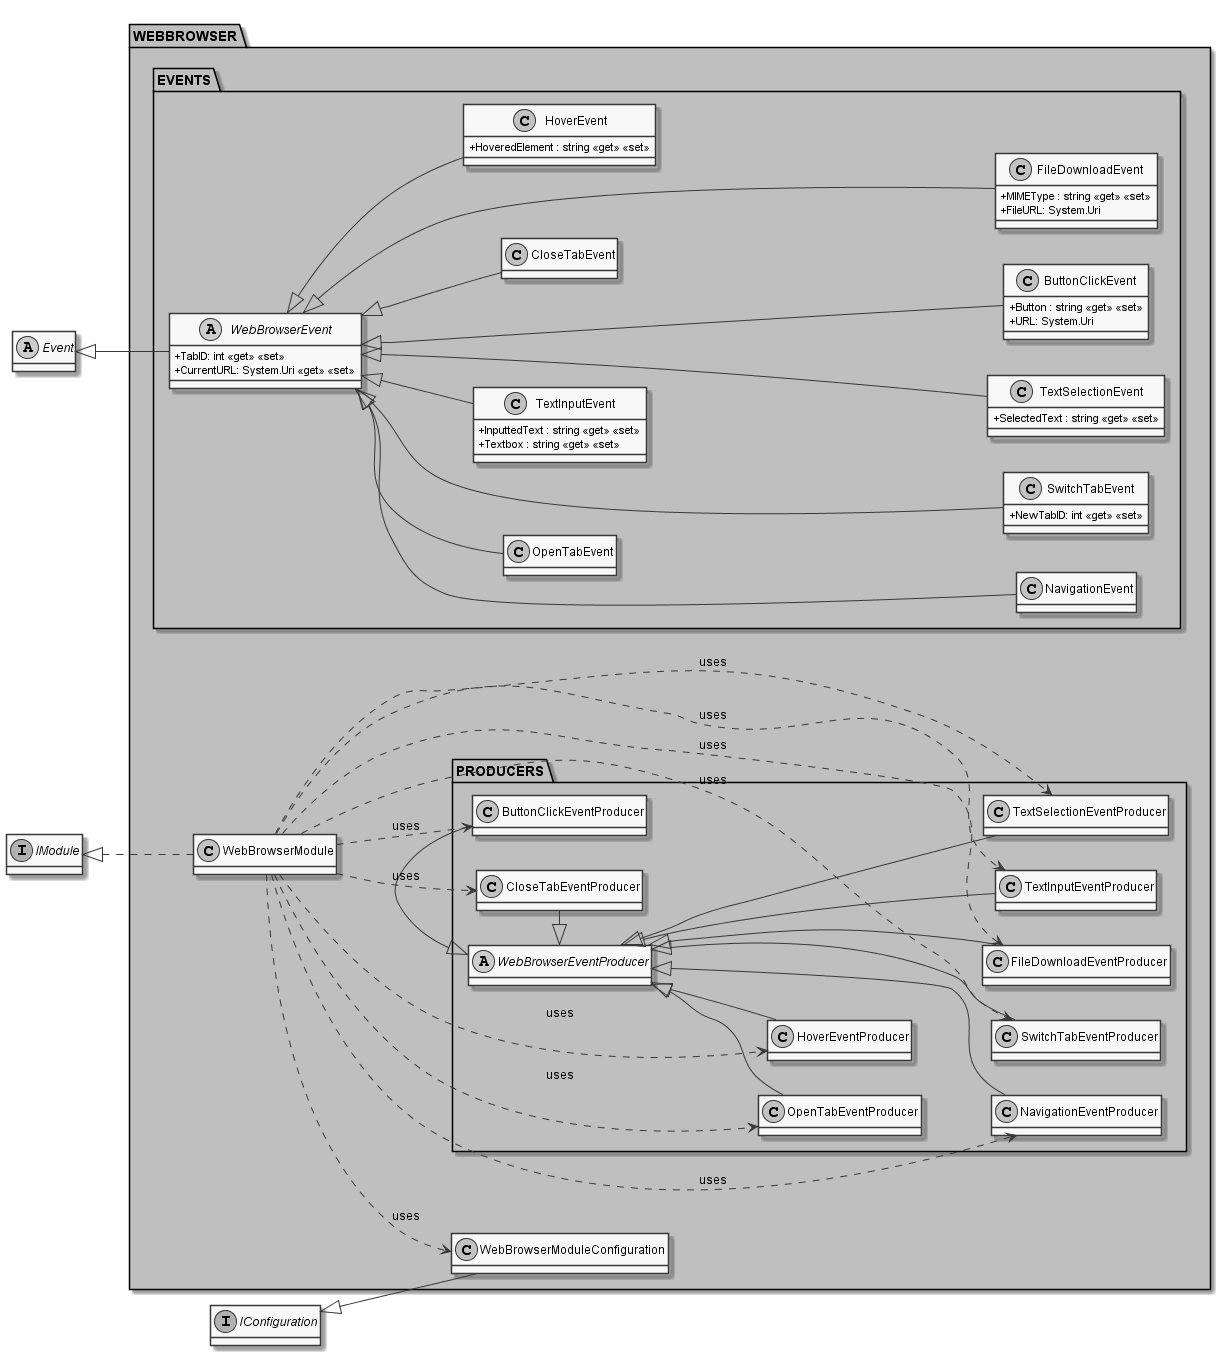
\includegraphics[width=1.0\textwidth]{resources/Packages/MODULES_WEBBROWSER.png}
\end{center}

The \textbf{MODULES.WEBBROWSER} package is responsible for providing the classes and concepts necessary for recording the webbrowser related user-interactions.

\begin{packclass}
\packobj{WebBrowserModule}
\packobj{\abstract{WebBrowserEvent}}
\packobj{TextSelectionEvent}
\packobj{TextInputEvent}
\packobj{SwitchTabEvent}
\packobj{OpenTabEvent}
\packobj{CloseTabEvent}
\packobj{NavigationEvent}
\packobj{HoverEvent}
\packobj{FileDownloadEvent}
\packobj{ButtonClickEvent}
\end{packclass}

\newpage
\subsection*{MORR.MODULES.CLIPBOARD}

\begin{center}
    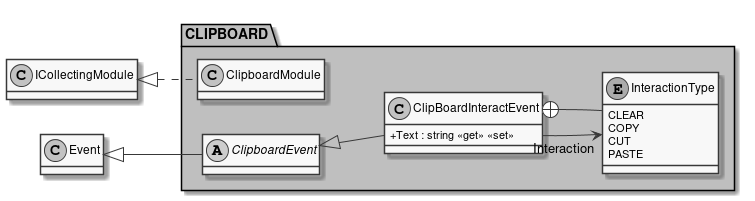
\includegraphics[width=1.0\textwidth]{resources/Packages/MODULES_CLIPBOARD.png}
\end{center}

The \textbf{MODULES.CLIPBOARD} package is responsible for providing the classes and concepts necessary for recording the clipboard related user-interactions.

\begin{packclass}
\packobj{ClipboardModule}
\packobj{\abstract{ClipboardEvent}}
\packobj{ClipBoardInteractEvent}
\end{packclass}

\begin{packenum}
\packobj{InteractionType}
\end{packenum}

\newpage
\subsection*{MORR.MODULES.MOUSE}

\begin{center}
    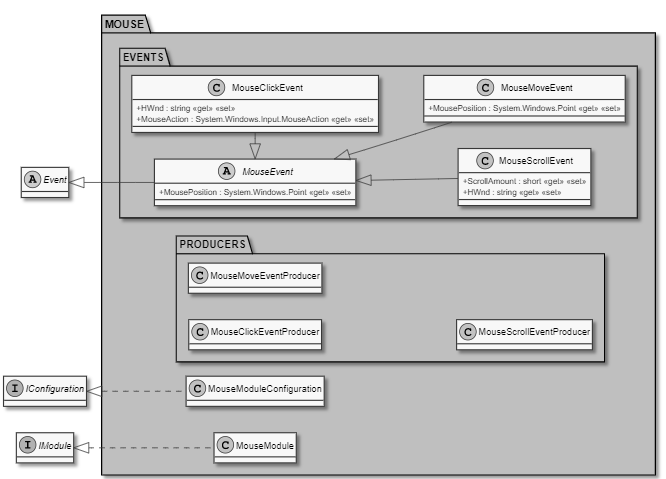
\includegraphics[width=1.0\textwidth]{resources/Packages/MODULES_MOUSE.png}
\end{center}

The \textbf{MODULES.MOUSE} package is responsible for providing the classes and concepts necessary for recording the mouse related user-inputs.

\begin{packclass}
\packobj{MouseModule}
\packobj{\abstract{MouseEvent}}
\packobj{MouseScrollEvent}
\packobj{MouseClickEvent}
\packobj{MouseMoveEvent}
\end{packclass}

\begin{packenum}
\packobj{MouseButton}
\packobj{MouseButtonState}
\end{packenum}
\newpage

\section{MORR.UI}

\begin{center}
    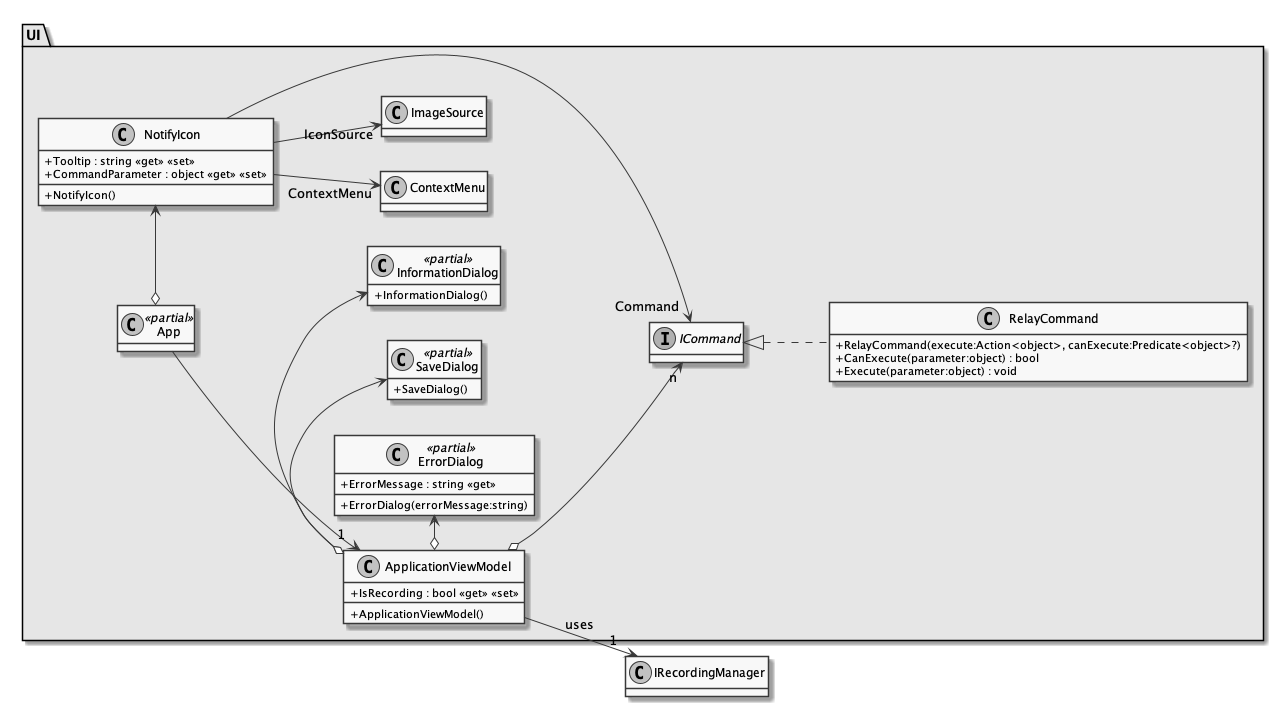
\includegraphics[width=1.0\textwidth]{resources/Packages/UI.png}
\end{center}

The \textbf{UI} package is responsible for the graphical user interface.

\begin{packclass}
\packobj{NotifyIcon}
\packobj{<<partial> App}
\packobj{<<partial>> InformationDialog}
\packobj{<<partial>> SaveDialog}
\packobj{<<partial>> ErrorDialog}
\packobj{ApplicationViewModel}
\packobj{RelayCommand}
\end{packclass}
         % package
\chapter{Classes}
\label{ch:class}           % Class design and description
\chapter{Dynamic diagrams}
\label{ch:dynamicdiagram}

\section{Core}
\subsection{Initialization of the core from the UI application}
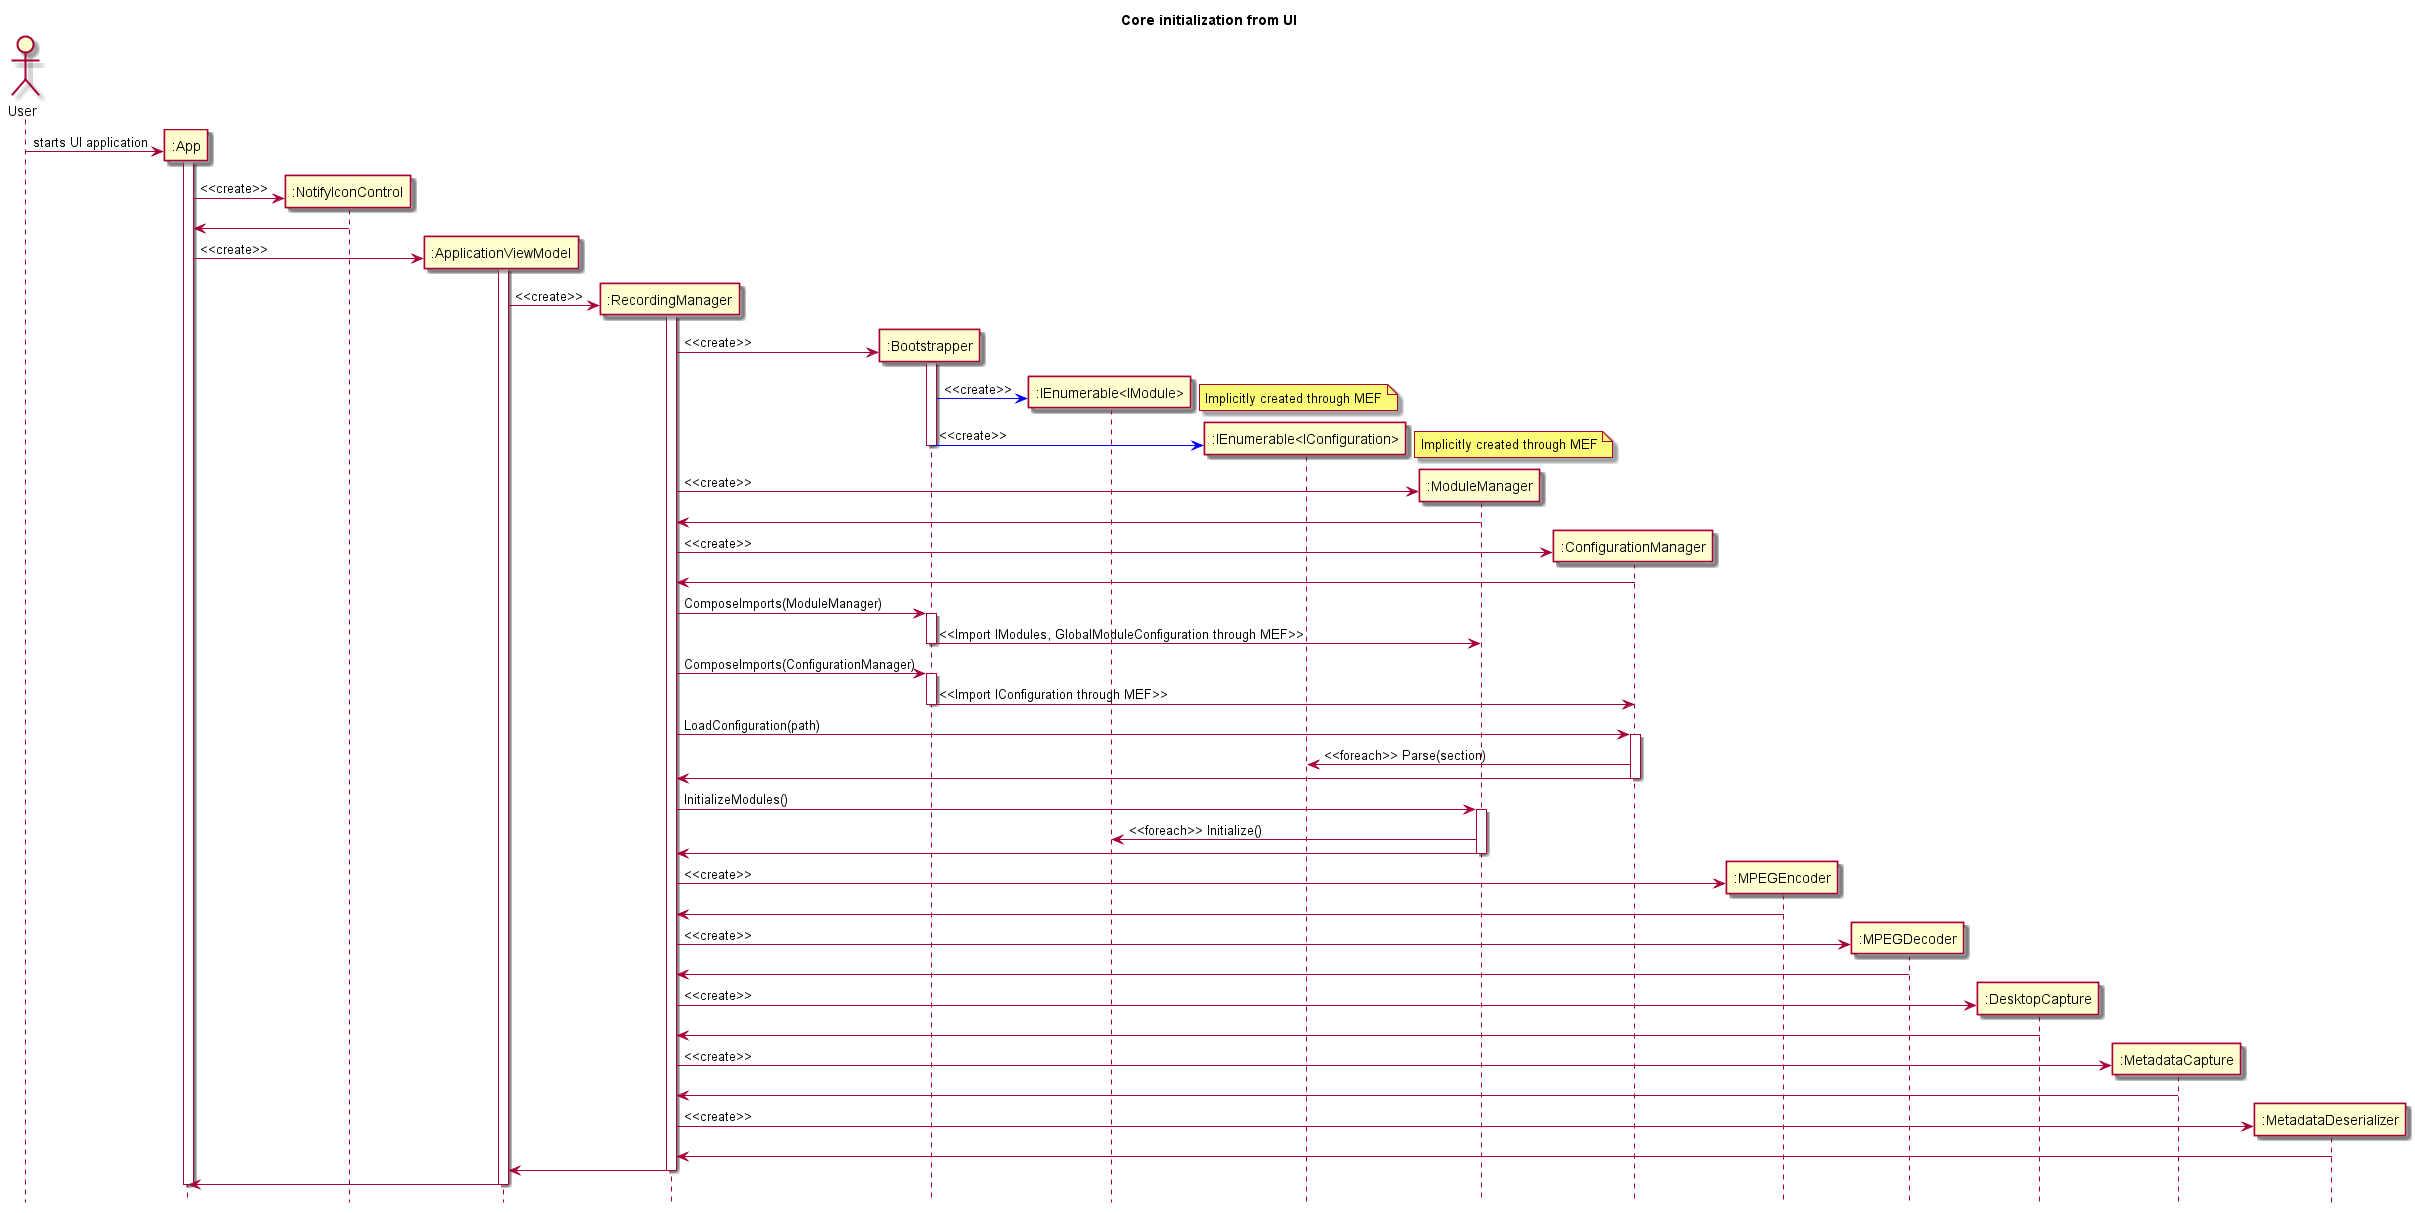
\includegraphics[width=1.0\textwidth]{resources/DynamicDiagrams/InitCore.png}
This diagram depicts the control flow when the user starts the UI application, up to the point where the core is ready for a recording to start.

\subsection{Event flow from keyboard module to the MPEG encoder}
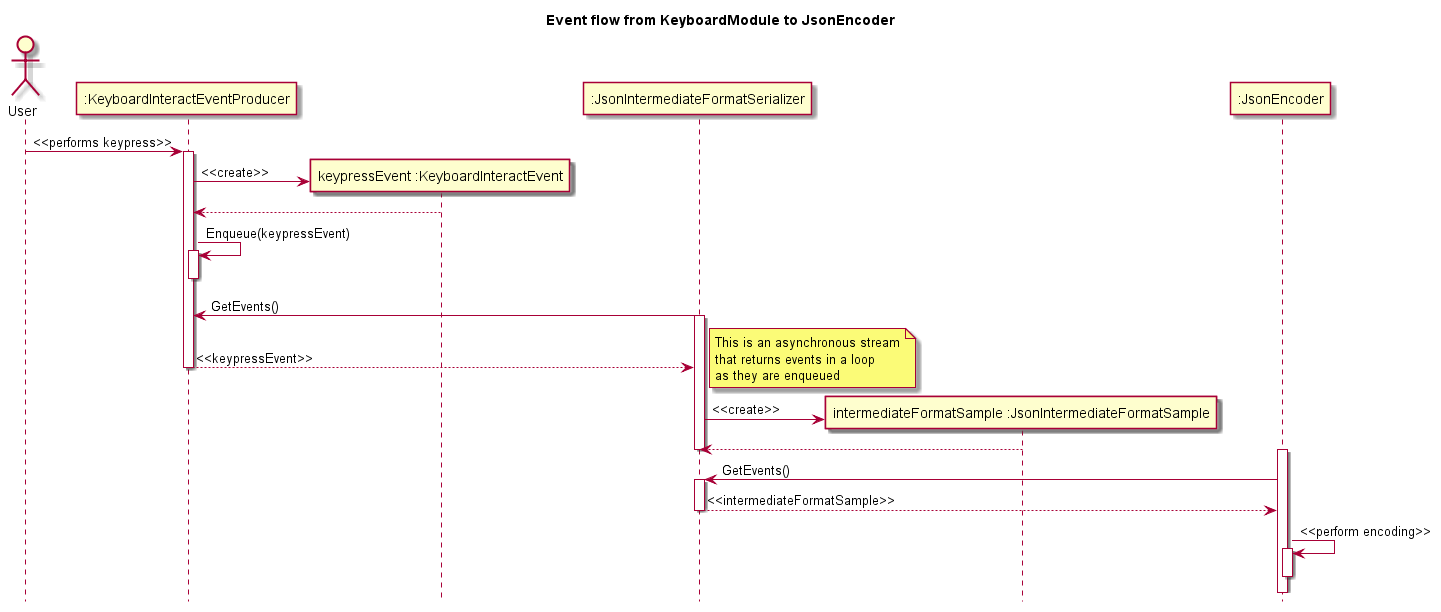
\includegraphics[width=1.0\textwidth]{resources/DynamicDiagrams/EventFlowKeyboardToEncoder.png}
This diagram depicts the control flow when the user presses a keyboard button, up to the point where the event has been encoded into the MPEG stream during a recording.

\section{Browser Extension}
\subsection{Initialization of the browser extension}
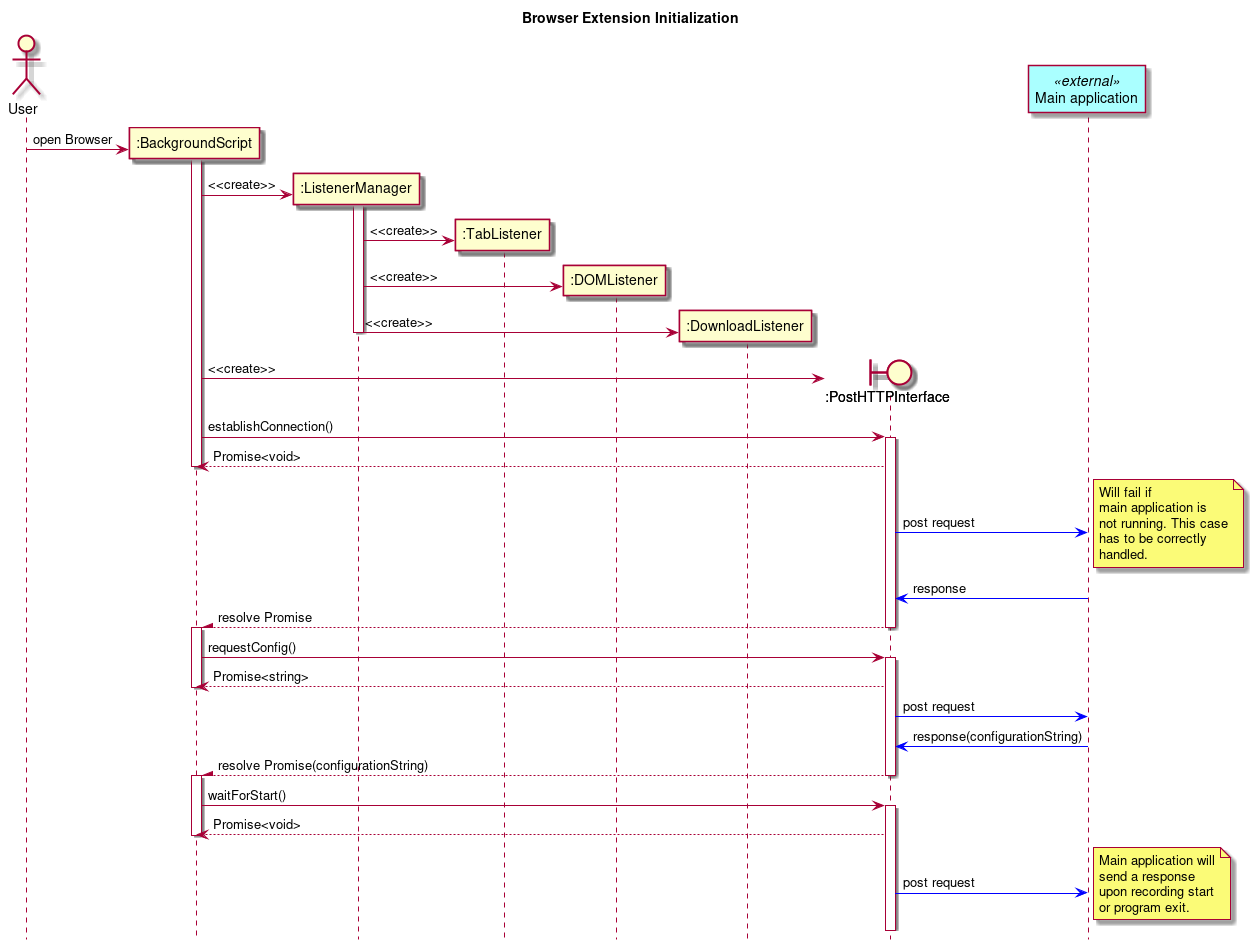
\includegraphics[width=1.0\textwidth]{resources/DynamicDiagrams/InitBrowserEx.png}
This diagram depicts the control flow when the browser is started and the browser extension initialized, up to the point where the browser extension is ready for a recording to start.

\subsection{Capturing a text selection event}
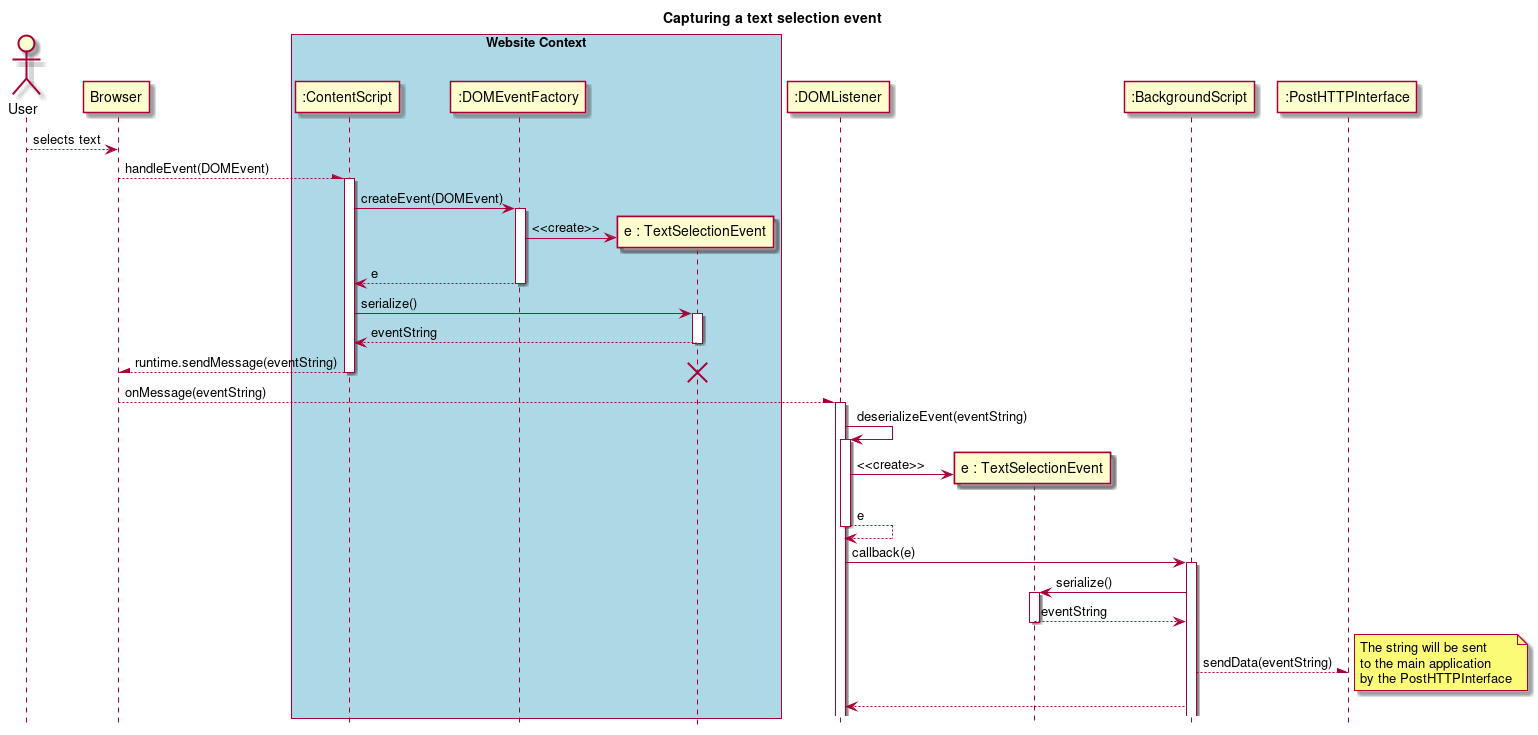
\includegraphics[width=1.0\textwidth]{resources/DynamicDiagrams/CaptureEvent.png}
This diagram depicts the control flow when the browser extension captures a text selection event during a recording. The control flow is described up to the point where the recorded event is handed over to the communication-interface which will attempt to send it to the main application. The control flow for other captured DOM events (meaning events occurring in the website-context) is identical.  % Dynamic diagrams
\chapter{Libraries}
\label{ch:libraries}

\newcommand{\lib}[2]{\item{\textbf{#1: }{#2}}}

This chapter provides an overview over the libraries that have been chosen for use in the application and the specific use cases that have been identified for them.

\subsection*{General}

\begin{itemize}
    \lib{.NET Core 3.1}{All C\# projects target .NET Core 3.1}
    \lib{.NET Framework}{All projects have access to the .NET Framework, which provides access to APIs related to Mouse/Keyboard devices and types related to Win32-specific objects}
    \lib{user32.dll}{Provides access to the Win32-API which exposes Mouse, Keyboard, Clipboard or Window events through message hooks}
\end{itemize}

\subsection*{CLI}

\begin{itemize}
    \lib{CommandLineParser}{Provides command line parsing for command line arguments}
\end{itemize}

\subsection*{MORR}

\begin{itemize}
    \lib{System.Composition}{Provides contract-based object imports/exports for dynamic composition}
    \lib{SharpDX.Direct3D11}{Provides C\#-friendly access to Direct3D11 utilized in screen capture}
\end{itemize}

\subsection*{UI}

\begin{itemize}
    \lib{WPF (version compatible with .NET Core 3 and later)}{Framework (not library) that provides UI-related objects}
\end{itemize}

\subsection*{BrowserExtension}

\begin{itemize}
    \lib{jQuery}{Provides methods for creation and sending of HTTP-Requests}
\end{itemize}		  % Libraries
\printnoidxglossaries
\end{document}
